\documentclass[twoside, a4paper, 12pt]{report}

\usepackage[utf8]{inputenc}
\usepackage[T1]{fontenc}
\usepackage[french]{babel}
\frenchbsetup{StandardLists=true} % on garde les belles puces

\usepackage{amsmath, amssymb, mathrsfs, stmaryrd, amsthm} % pr les maths
\usepackage{graphicx,caption} % pr image
\usepackage[hidelinks]{hyperref}  % sommaire cliquable
\usepackage{url}

\usepackage{listings} % pour code source
\usepackage{color}
\definecolor{deepblue}{rgb}{0,0,0.5}
\definecolor{deepred}{rgb}{0.6,0,0}
\definecolor{deepgreen}{rgb}{0,0.5,0}
\DeclareFixedFont{\ttb}{T1}{txtt}{bx}{n}{12} % for bold
\DeclareFixedFont{\ttm}{T1}{txtt}{m}{n}{12}  % for normal
\lstset{
breaklines=true,
numbers=left,
language=Python,
basicstyle=\ttm,
otherkeywords={self},             % Add keywords here
keywordstyle=\ttb\color{deepblue},
emph={MyClass,__init__},          % Custom highlighting
emphstyle=\ttb\color{deepred},    % Custom highlighting style
stringstyle=\color{deepgreen},
frame=tb,                         % Any extra options here
showstringspaces=false            % 
}


\usepackage[top=1cm, bottom=2cm, left=1cm, right=1cm]{geometry}
% \usepackage{subfig}
\usepackage{subcaption}
\usepackage{pdfpages} %img full

\title{Problème du Serpent \\ Dénombrement de chaînes dans un graphe rectangle}
\author{Théo \textsc{Rudkiewicz} }
\date{\today}

\newtheorem*{lemma}{Lemme} % La petite étoile enlève la numérotation, maisnécessite le package amsthm
\newtheorem{theorem}{Théorème}[chapter]
\newtheorem{property}[theorem]{Proposition}    
\newtheorem{definition}{Définition}[chapter] % Le [chapter] peut par exemple êtreremplacé par [section], il permet de numéroter les éléments par rapport aux numéros de chapitre
\newtheorem{corollary}{Corollaire}[theorem]
\newtheorem{conjecture}{Conjecture}


\renewcommand\qedsymbol{$\blacksquare$}  % change le carré de fin de démo

% \usepackage{thmtools}
% \renewcommand{\listtheoremname}{List of theorems and definitions}

\usepackage{shorttoc}


\newcommand{\pythonlogo}{
\includegraphics[width=1em , height=2ex]{python128.png}}
\newcommand{\cqfd}[1][\quad]{\ensuremath{#1\blacksquare}}
\newcommand{\subcqfd}[1][\quad]{\ensuremath{#1\square}}

\newcommand{\parite}[1]{\ensuremath{\text{Parité}(#1)}}
\newcommand{\parcours}[2]{\ensuremath{\text{Parcours}(#1 \times #2)}}
\newcommand{\trajet}[6]{\ensuremath{\text{Trajet}\left(#1 \times #2; (#3, #4); (#5; #6)\right)}}
\newcommand{\pa}[2]{\ensuremath{\text{P}_A\left(#1 \times #2\right)}}
\newcommand{\pb}[2]{\ensuremath{\text{P}_B\left(#1 \times #2\right)}}
\newcommand{\po}[2]{\ensuremath{\text{P}_O\left(#1 \times #2\right)}}
\newcommand{\Pm}[1]{\ensuremath{\text{P}_M\left(#1\right)}}
\newcommand{\Pmtot}[1]{\ensuremath{\text{Parcours}_M\left(#1\right)}}
\newcommand{\Pc}[1]{\ensuremath{\text{P}_{C\uparrow}(#1)}}
\newcommand{\Pctot}[1]{\ensuremath{\text{Parcours}_C(#1)}}

\begin{document}

\includepdf{serpent_couv_1.pdf}
\newpage
\null
\thispagestyle{empty}
\newpage
\maketitle
\shorttoc{Sommaire}{1}
% \setcounter{tocdepth}{2}
% \tableofcontents


\chapter{Introduction}

On cherche à dénombrer l'ensemble des chaînes hamiltoniennes orientées dans un graphe rectangle de taille $L \times l$. (cf Fig \ref{graphe_4_5})

En utilisant des listes, structure plus adaptée à une implémentation, on peut définir le problème comme suit.
Un parcours est une liste ordonnée de positions. Soit $P$ un parcours. $L \times l$ est la taille du graphe.
\[
P \text{ est valide} \Longleftrightarrow
\left\{
    \begin{array}{ll}
        (1) \forall (x, y) \in \llbracket 1; L \rrbracket \times \llbracket 1; l \rrbracket; (x, y) \in P\ \ (\text{Tout les points sont atteints})\\
        (2) \forall p \in P; p \in \llbracket 1; L \rrbracket \times \llbracket 1; l \rrbracket\ \   (\text{Rien ne dépasse du carré})\\
	    (3) \forall (p, q) \in P^2; p \ne q\ \  (\text{Aucun point n'est atteint deux fois})\\
        (4) \forall i \in \llbracket 1; L \times l \rrbracket / P_i = (x, y);  [P_{i+1} = (x \pm 1, y)] \lor[P_{i+1} = (x, y\pm1)] \\(\text{Tout les déplacements sont justes})\\
    \end{array}
\right.
\]

On cherche $\text{max}(\text{card}(\Omega))$
\[ \Omega = \bigcup P / P\text{ est valide} \]

\begin{figure}[h]
\centering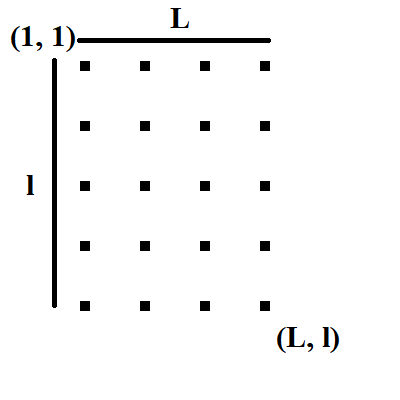
\includegraphics[scale=0.7]{graphe(4_5)_2.png}
\caption{Représentation du graphe  $4 \times 5$}
\label{graphe_4_5}
\end{figure}

\begin{figure}[h]
\centering
\includegraphics[scale=5]{graphes_2x2.png}
\caption{Représentation de $\Omega$ pour $G(2\times2)$}
\label{parcours_c2}
\end{figure}

\begin{figure}[h]
\centering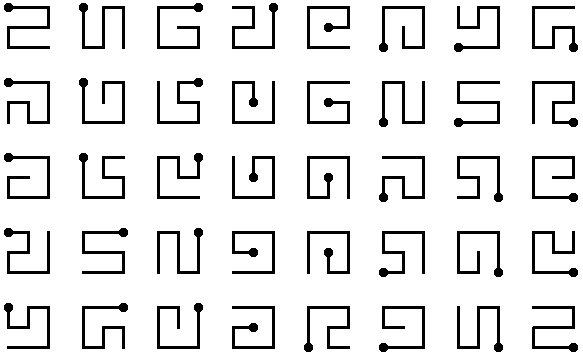
\includegraphics[scale=0.8]{Serpent.png}
\caption{Représentation de $\Omega$ pour  $G(3\times3)$}
\label{parcours_c3}
\end{figure}

\section{Définitions}

\begin{itemize}

\item On note $G(L \times l)$ le graphe rectangle de taille $L$ par $l$. Par convention, on note $G'$ les sous-graphes.
\item On attribue des coordonnées à chaque point. La première est l'avancement sur la longueur $L$ (par convention horizontale vers la droite). La deuxième est l'avancement sur la largeur $l$ (par convention verticale vers le bas). Ainsi les coordonnées vont de $(1,1)$ à $(L, l)$.

\item 
On utilise par la suite certaines dénominations pour des motifs précis:
\begin{itemize}
\item  en colimaçon 
\includegraphics[scale=1]{colimacon.png}
\item en direct 
\includegraphics[scale=1]{direct.png}
\end{itemize}

\item 
\[
\text{Trajet}
\left|
  \begin{array}{rcl}
    {\left(\mathbb{N^*}^2\right)}^3  &\longrightarrow & \mathbb{N} \\
    (L \times l); (x, y); (\chi, \upsilon) & \longmapsto& \text{Nombre de parcours de } (x; y) \text{ vers } (\chi; \upsilon) \text{ dans le graphe } G(L \times l)\\
  \end{array}
\right.
\]

\item \[\trajet{L}{l}{x}{y}{\lambda}{\lambda} = \trajet{L}{l}{\lambda}{\lambda}{x}{y}  = \sum_{\chi = 1; \upsilon = 1}^{\chi = L;\upsilon = l}\trajet{L}{l}{x}{y}{\chi}{\upsilon}\]
\item \[\parcours{L}{l} = \sum_{x = 1; y = 1}^{x = L; y = l}\trajet{L}{l}{x}{y}{\lambda}{\lambda}\]
\item $\pa{L}{l} = \trajet{L}{l}{1}{1}{\lambda}{\lambda}$
\item $\pb{L}{l} = \trajet{L}{l}{1}{1}{L}{1} \not= \pb{l}{L} = \trajet{L}{l}{1}{1}{1}{l}$
\item $\po{L}{l} = \trajet{L}{l}{1}{1}{L}{l}$

\item Une case de coordonnées $(x, y)$ est dite paire si et seulement si $x + y$ est paire et impaire si et seulement si $x + y$ est impaire.
 \[
\text{Parité}
\left|
  \begin{array}{rcl}
    \mathbb{N}^2  &\longrightarrow &\{0; 1\} \\
    (x, y) & \longmapsto& (x + y) \% 2\\
  \end{array}
\right.
\]

\item Un chemin, contrairement à un parcours ne prend pas en compte le sens dans lequel le serpent est mis. Ainsi: $[(0,0); (1,0)] \Leftrightarrow [(1,0) ; (0,0)]$. Il s'agit alors d'une chaîne hamiltonienne dans un graphe non orienté.
\end{itemize}


\chapter{Cas d'un graphe rectangle quelconque}
\section{Parité}
\subsection{Lemme : répartition de la parité}

\begin{lemma}
 \[
2 \nmid L \times l \Leftrightarrow
\left\{
    \begin{array}{ll}
        \text{nombre de cases paires} = \frac{L \times l + 1}{2}\\
        \text{nombre de cases impaires} = \frac{L \times l - 1}{2} \subcqfd
    \end{array}
\right.
\]
 \[
2 \mid L \times l \Leftrightarrow \text{nombre de cases paires} = \text{nombre de cases impaires} = \frac{L \times l }{2} \subcqfd
\]
\end{lemma}

\subsection{Théorème parité}

\begin{theorem}[Théorème parité] \label{theoreme_parite}
\begin{enumerate}\ \\
\item \label{prop_changement_parite}
\[ \forall i \in \llbracket 1; L \times l \rrbracket; \parite{P_i} \not = \parite{P_{i+1}} \] 
\item 
\[
\left\{
    \begin{array}{ll}
        2 \mid L \times l \Leftrightarrow \parite{P_0} \not= \parite{P_{-1}}\\
        2 \nmid L \times l \Leftrightarrow \parite{P_0} = \parite{P_{-1}}
    \end{array}
\right.
\]
\end{enumerate}
\end{theorem}

% \subsubsection{Démonstrations}

\begin{enumerate}
\item
\begin{proof}
D'après la définition d'un parcours valide: 
\[(4) \forall i \in \llbracket 1; L \times l \rrbracket / P_i = (x, y);  [P_{i+1} = (x \pm 1, y)] \lor[P_{i+1} = (x, y\pm1)] \\(\text{Tout les déplacements sont justes})\]
Or $x + y \not \equiv (x + y) \pm 1 [2]$ donc:
\[ \forall i \in \llbracket 1; L \times l \rrbracket; \parite{P_i} \not = \parite{P_{i+1}}\] 
\end{proof}

\item
\begin{proof}
Dans $G(L \times l)$, il y a $L \times l - 1$ arêtes empruntées, or d'après la propriété (\ref{prop_changement_parite}), cela corespond à $L \times l - 1$ changement de parité. Les changements de parités s'annulent deux à deux donc seul la parité du nombre de changements compte. Ainsi si le nombre de changements est pair, la parité est conservée sinon elle est inversée. D'où:
\[
\left\{
    \begin{array}{lll}
        2 \nmid L \times l - 1 \Leftrightarrow 2 \mid L \times l \Leftrightarrow \parite{P_0} \not= \parite{P_{-1}}\\
       2 \mid L \times l  - 1\Leftrightarrow  2 \nmid L \times l \Leftrightarrow \parite{P_0} = \parite{P_{-1}} 
    \end{array}
\right.
\]
\end{proof}
\end{enumerate}



\subsection{Application du théorème parité aux graphes impairs}

\begin{corollary}[Départs imposssibles] \label{coro_th_parite}
\[ 2 \nmid L \times l \Leftrightarrow \lnot \exists P/ (P \text{ est valide} \land \parite{P_0} = 1) \]
\end{corollary}
\begin{figure}[h!]
\centering
\includegraphics[scale=5]{graphe(5_5)_marquer.png}
\caption[Application du corollaire \ref{coro_th_parite} au graphe carré $5 \times 5$]{Application du corollaire \ref{coro_th_parite} au graphe carré $5 \times 5$ (avec en rouge les cases d'où aucun parcours ne part)}
\label{graphe_carre_impossible_c5}
\end{figure}

\begin{proof}
Par l'absurde :
On suppose qu'il existe un parcours partant d'une case impaire allant vers une case impaire.
Entre ces deux points il devra parcourir $\frac{L \times l + 1}{2}$ case paires et $\frac{L \times l - 1}{2} - 2$ case impaires.
Or le parcours est forcément constitué d'une alternance de cases paires et impaires. Ce trajet n'existe donc pas.

\end{proof}

\section{Théorème réducteur} \label{theoreme_reducteur}

\begin{theorem}[Théorème Réducteur]
\begin{enumerate}

\item Réduction simple: 
\[\forall (L; l) \in \mathbb{N^*}^2; \pa{L}{l} \geq \pa{L}{l-1} + \pa{L-1}{l}\]

\item Réduction en colimaçon impairs: 
\begin{enumerate}
\item $\forall (L; l) \in \mathbb{N^*}^2 /( 2\nmid L);$
\[ \pa{L}{l} \geq Red(l) + \sum_{h=1}^{l-1}\pa{L}{h}\]

\item $\forall (L; l) \in \mathbb{N^*}^2 /( 2\nmid l);$
\[ \pa{L}{l} \geq Red(L) + \sum_{h=1}^{L-1}\pa{h}{l}\]
\end{enumerate}

\item Réduction en colimaçon pairs:

\begin{enumerate}
\item $\forall (L; l) \in \mathbb{N^*}^2 / (2\mid L);  $
\[\pa{L}{l} \geq Red(l) + \pa{L}{l-1} + \sum_{h=1}^{l-2}\sum_{x=1; 2 \nmid x}^{L-1} \trajet{L}{h}{1}{1}{x}{1}\]

\item $\forall (L; l) \in \mathbb{N^*}^2 / (2\mid l); $
\[\pa{L}{l} \geq Red(L) + \pa{L-1}{l} + \sum_{h=1}^{L-2}\sum_{x=1; 2 \nmid x}^{l-1} \trajet{h}{l}{1}{1}{1}{x}\]
\end{enumerate}

\item Réduction combinnées:

\begin{enumerate}
\item $ \forall (L; l) \in \left(2\mathbb{N^*}\right)^2 ; \pa{L}{l} \geq$
\[  \sum_{h=1}^{L-1}\pa{h}{l} + \sum_{h=1}^{l-1}\pa{L}{h}\]

\item $ \forall (L; l) \in \mathbb{N^*}^2 / (2\mid L \land 2\mid l) ; \pa{L}{l} \geq$
\[ \pa{L}{l-1} + \sum_{h=1}^{l-2}\sum_{x=1; 2 \nmid x}^{L-1} \trajet{L}{h}{1}{1}{x}{1} \\
+ \pa{L-1}{l} + \sum_{h=1}^{L-2}\sum_{x=1; 2 \nmid x}^{l-1} \trajet{h}{l}{1}{1}{1}{x}\]

\item $ \forall (L; l) \in \mathbb{N^*}^2 / (2\nmid L \land 2\mid l); \pa{L}{l} \geq$
\[  \sum_{h=1}^{l-1}\pa{L}{h} + \pa{L-1}{l} + \sum_{h=1}^{L-2}\sum_{x=1; 2 \nmid x}^{l-1} \trajet{h}{l}{1}{1}{1}{x}\]

\item $ \forall (L; l) \in (2\mathbb{N^*} + 1)^2; \pa{L}{l} \geq$
\[  \pa{L}{l-1} + \sum_{h=1}^{l-2}\sum_{x=1; 2 \nmid x}^{L-1} \trajet{L}{h}{1}{1}{x}{1} + \sum_{h=1}^{l-1}\pa{L}{h}\]
\end{enumerate}

\end{enumerate}
\end{theorem}

\begin{proof}
\begin{enumerate}
\item On cherche à montrer que l'on peut se ramener au parcours d'un sous-graphe. On part ainsi d'un graphe $G(L \times l)$ et on le réduit à un graphe $G'(L \times l-1)$. On peut effectuer cette réduction en longeant simplement le bord (cf Fig. \ref{red_simple}). Ainsi on peut effectuer cette réduction des deux cotés. On a alors à parcourir $G'(L \times l-1)$ et $G'(L-1 \times l)$. De plus, ces deux réductions sont compatibles donc elles ne compteront pas deux fois la même chose. D'où: 
\[\forall (L; l) \in \mathbb{N^*}^2; \pa{L}{l} \geq \pa{L}{l-1} + \pa{L-1}{l} 
\cqfd\]

\begin{figure}[h]
\centering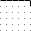
\includegraphics[scale=5]{red_simple.png}
\caption[Réduction au parcours du sous-graphe $G'(L\times l-1)$]{Réduction au parcours du sous-graphe $G'(L\times l-1)$ (en vert foncé le départ et en vert clair le nouveau départ)}
\label{red_simple}
\end{figure}

\item On cherche à montrer l'on peut se ramener au parcours d'un ensemble de sous-graphe. $L$ est impair donc on peut réduire par colimaçon (cf Fig. \ref{red_impair_coli}). Pour réduire aux sous-graphes $G'(L \times l-2)$, $G'(L \times l-3)$, ..., $G'(L \times 1)$. On peut également effectuer cette réduction à partir du côté $l$. De plus, ces réductions sont compatibles avec la réduction simple et compatibles entre elles. D'où:
\[\left\{\begin{array}{ll}
\forall (L; l) \in \mathbb{N^*}^2 /( 2\nmid L); \pa{L}{l} \geq Red(l) + \sum_{h=1}^{l-1}\pa{L}{h}\\
\forall (L; l) \in \mathbb{N^*}^2 /( 2\nmid l); \pa{L}{l} \geq Red(L) + \sum_{h=1}^{L-1}\pa{h}{l}
\end{array}\right. 
\cqfd\]

\begin{figure}[h]
\centering
\includegraphics[scale=5]{red_impair_coli.png}
\caption[Réduction au parcours du sous-graphe  $G'(L\times l-3)$]{Réduction au parcours du sous-graphe  $G'(L\times l-3)$ (en vert foncé le départ et en vert clair le nouveau départ)}
\label{red_impair_coli}
\end{figure}

\item Dans le cas d'une longueur impaire, une réduction par colimaçon laisse forcément un trou (cf Fig. \ref{red_pair_coli}). Ce trou doit forcément être le point d'arrivée car il y est impossible de faire demi-tour. De plus ce trou ne peut être présent à n'importe quel point : il sera forcément impair pour satisfaire le théorème de parité (cf. \ref{theoreme_parite}). Ainsi le départ et l'arrivée du parcours sont fixés. D'où:
\[\left\{\begin{array}{ll}
\forall (L; l) \in \mathbb{N^*}^2 / (2\mid L); \pa{L}{l} \geq Red(l) + \pa{L}{l-1} + \sum_{h=1}^{l-2}\sum_{x=1; 2 \nmid x}^{L-1} \trajet{L}{h}{1}{1}{x}{1}\\
\forall (L; l) \in \mathbb{N^*}^2 / (2\mid l); \pa{L}{l} \geq Red(L) + \pa{L-1}{l} + \sum_{h=1}^{L-2}\sum_{x=1; 2 \nmid x}^{l-1} \trajet{h}{l}{1}{1}{1}{x}
\end{array}\right. 
\cqfd\]

\begin{figure}[h]
\centering
\includegraphics[scale=5]{red_pair_coli.png}
\caption[Réduction au parcours du sous-graphe $G'(L\times l-3)$ avec arrivée contrainte]{Réduction au parcours du sous-graphe $G'(L\times l-3)$ avec arrivée contrainte (en vert foncé le départ et en vert clair le nouveau départ, en rouge le départ et en orange la nouvelle arrivée)}
\label{red_pair_coli}
\end{figure}

\item Les réductions paires sur un côté et impaires de l'autre ne peuvent aboutir au même trajet. Par exemple, si l'on réduit de façon impaire de 3 la longueur $L$ et de 5 la largeur $l$ aucun des parcours de la première réduction ne seront possibles après la seconde.  \cqfd
\end{enumerate}
\end{proof}

\chapter{Graphe $n \times 1$}

\begin{property}
\begin{align}
\forall n \in \mathbb{N^*};& \pa{1}{n} = 1 \subcqfd \\
\forall n \in \mathbb{N^*};& \po{1}{n} = 1 \subcqfd \\
\forall n \in \mathbb{N^*} \backslash \{1\}; &\pb{1}{n} = 0 \subcqfd \\
\forall n \in \mathbb{N^*}; & \pb{n}{1} = 1 \subcqfd \\
\forall n \in \mathbb{N^*}; &\parcours{1}{n} = 2 \subcqfd
\end{align}
\end{property}

\chapter{Graphe $n \times 2$}

\section{Nombre de parcours à partir d'un angle}

\begin{property}[\pa{n}{2}]\label{pa_n_2}
Quel que soit un point atteignable (d'après le théorème parité) à partir de l'angle, il existe un unique parcours qui arrive à ce point.
\[\forall n \in \mathbb{N}^*; \pa{n}{2} = n\]
\end{property}

\begin{property}\label{pb_po_n_2}
\begin{itemize}
\item $\pb{2}{L} = 1$

\item 
Si $2 \mid n$:
$\pb{L}{2} = 1$ \\
Si $2 \nmid n$:
$\pb{L}{2} = 0$

\item
Si $2 \mid n$:
$\po{L}{2} = 0$ \\
Si $2 \nmid n$:
$\po{L}{2} = 1$
\end{itemize}
\end{property}

\begin{proof}[Démonstration de la propriété \ref{pa_n_2}]
Au premier point il y a deux situations possibles:
\begin{itemize}
\item partir vers la droite et donc aller jusqu'à l'autre extrémité pour pouvoir atteindre la case sur le bord opposé de la case de départ, c'est un parcours direct, on atteint alors le seul point atteignable d'après le théorème parité. (cf Fig. \ref{direct_u})
\begin{figure}[h]
\centering
\includegraphics[angle=90, scale=5]{direct_u.png}
\caption{Parcours direct en U}
\label{direct_u}
\end{figure}
\item faire un motif d'escalier et se retrouver dans exactement la même situation avec un sous-graphe $G'(n-1\times 2)$ à parcourir. On ne peut alors plus atteindre le point non-atteingnable d'après le théorème de parité de la deuxième ligne. (cf Fig. \ref{reduction})
\begin{figure}[h]
\centering
\includegraphics[angle=90, scale=5]{reduction.png}
\caption[Réduction au parcours du sous-graphe $G'(n-1\times 2)$]{Réduction au parcours du sous-graphe $G'(n-1\times 2)$ (en vert foncé le départ et en vert clair le nouveau départ)}
\label{reduction}
\end{figure}
\end{itemize}
On a alors que $\pa{n+1}{2} = 1 + \pa{n}{2}$. Il s'agit ici de l'application stricte du théorème réducteur simple. (cf \ref{theoreme_reducteur}). Par ailleurs dans le cas où $n=1$, il y a un seul trajet à partir d'une extrémité donc $\pa{2}{1} = 1$. Par récurrence; $\forall n \in \mathbb{N}^*; \pa{2}{n} = n$. De plus, on remarque que tous les points que le théorème parité ne rend pas inatteignable sont atteints une unique fois (ce qui est confirmé par le nombre de point atteignables $\frac{n \times 2}{2} = n = \pa{2}{n}$).
\end{proof}

\begin{proof}[Démonstration de la propriété \ref{pb_po_n_2}]
\begin{itemize}

Le graphe est pair: $2 \mid L \times 2 \Leftrightarrow \parite{P_0} \not= \parite{P_{-1}}$.

\item Le point à atteindre pour \pb{2}{L} est de coordonnée $(1, 2)$ donc de parité impaire, d'où:
\[\pb{2}{L} = 1\]

\item Le point à atteindre pour \pb{L}{2} est de coordonnée $(L, 1)$ donc de parité inverse à L, d'où:
Si $2 \mid n$:
$\pb{L}{2} = 1$ \\
Si $2 \nmid n$:
$\pb{L}{2} = 0$

\item Le point à atteindre pour \po{L}{2} est de coordonnée $(L, 2)$ donc de même parité que L, d'où:
Si $2 \mid n$:
$\po{L}{2} = 0$ \\
Si $2 \nmid n$:
$\po{L}{2} = 1$
\end{itemize}
\end{proof}

\section{Parcours depuis un côté}

\begin{property}[Parcours depuis un côté]
\[\forall h \in \mathbb{N}^* \backslash \{1; n\};      \trajet{n}{2}{h}{1}{\lambda}{\lambda} = \trajet{n}{2}{h}{2}{\lambda}{\lambda} = n - 1\]
\end{property}

\begin{proof}
A partir d'un point lambda, on est obligé de partir parcourir soit la partie au dessus soit celle du dessous. De plus ce parcours doit s'effectuer en direct pour ne pas couper le graphe en deux parties incomplètes. Lors qu'on revient un cran plus loin que le point de départ, on arrive alors sur l'extrémité d'un sous-graphe à parcourir.  (cf Fig.\ref{reduction_alternative})
\begin{figure}[h!]
\centering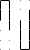
\includegraphics[angle=90, scale=5]{reduction_alternative.png}
\caption[Réduction au parcours de deux nouveaux sous-graphes : $G'(n-h\times 2)$ et de $G'(h-1\times 2)$]{Réduction au parcours de deux nouveaux sous-graphes : $G'(n-h\times 2)$ et de $G'(h-1\times 2)$ (en vert foncé le départ et en vert clair le nouveau départ)}
\label{reduction_alternative}
\end{figure}

Par conséquent le nombre de parcours pour un point est la somme du nombre de parcours dans les deux sous-graphes $G'(n-h\times 2)$ et $G'(h-1\times 2)$, ces parcours s'effectuent à partir d'une extrémité d'où:
\[\trajet{n}{2}{h}{1}{\lambda}{\lambda}  = \pa{n - h}{2} + \pa{h-1}{2} = n - h + h - 1 = n - 1\]
\end{proof}

\section{Conclusion}
\begin{theorem}[\parcours{n}{2}]
$$\forall n \in \mathbb{N^*} \backslash \{1\}; \parcours{n}{2} = 2(n^2 - n + 2)$$
\end{theorem}

\begin{proof}
Pour $ n > 1$, il y a 4 angles et 2 côtés sur chaque côté il y a $n - 2$ points qui ne sont pas des angles. On a alors:
\begin{align}
\forall n \in \mathbb{N^*} \backslash \{1\}; \parcours{n}{2} &= 4\times\pa{n}{2} + 2(n-2)\times\trajet{n}{2}{h}{1}{\lambda}{\lambda} \\
&= 4n + 2(n-2)(n-1) \\
&= 2(n^2 - n + 2)
\end{align}
\end{proof}


\chapter{Graphe $n \times 3$}

\section{\pb{3}{n}}

\begin{property}[\pb{3}{n}]\ \newline \label{prop_pb_3_n}

\begin{enumerate}
\item Si $2 \mid n$: \[\pb{3}{n} = 0\]
\item Sinon alors $2 \nmid n$: \[\pb{3}{n} = 2^{\frac{n-1}{2}}\]
\end{enumerate}
\end{property}

\begin{proof}
\begin{enumerate}
\item \[2 \mid n \Leftrightarrow 2 \mid 3n \Leftrightarrow \parite{P_0} \not= \parite{P_{-1}}\]
Or on cherche à aller de $(1; 1)$ à $(1; 3)$. Or $\parite{(1, 1)} = \parite{(3, 3)}$ donc d'après le théorème parité (cf \ref{theoreme_parite}), c'est impossible :
\[\pb{3}{n} = 0 \]

\item $2 \nmid n$ donc on peut faire un parcours en colimaçon le long d'un coté ou de l'autre en descendant puis remontant. On montre alors qu'il y a exactement $\frac{n-1}{2}$ motifs à répartir d'un coté ou de l'autre (cf Fig. \ref{pb_3_n}) On utilise les méthodes de dénombrement classique et on obtient :
\[\pb{3}{n} = 2^{\frac{n-1}{2}}\]
\end{enumerate}
\end{proof}

\begin{figure}[h]
\begin{center}
\begin{subfigure}[b]{0.1\textwidth}
   
\includegraphics[width=1\linewidth, scale=1]{3_5_pb_3n_v1.png}
   \caption{Version (Gauche, Droite)}
\end{subfigure} \hspace{5cm}%
\begin{subfigure}[b]{0.1\textwidth}
   
\includegraphics[width=1\linewidth, scale=1]{3_5_pb_3n_v2.png}
   \caption{Version (Gauche,  Gauche)}
\end{subfigure}
\caption{Deux parcours pour \pb{3}{n}}
\label{pb_3_n}
\end{center}
\end{figure}


\section{\pb{n}{3}; \po{n}{3}}
\subsubsection{Propriétés}
\begin{enumerate}
\item Lemme arithmétique:
\[1 + \sum_{k=0}^{n-1} 2^k = 2^n  \subcqfd\]
\item \[\pb{1}{3} = 0; \po{1}{3} = 1 \subcqfd\]
\item \[\forall n \in \mathbb{N^*}; \pb{n}{3} = \sum_{h=1}^{n-1} \po{h}{3}\]
\item \[\forall n \in \mathbb{N^*}; \po{n}{3} = 1 + \sum_{h=1}^{n-1} \pb{h}{3}\]
\item \[\forall n \in \mathbb{N^*} \backslash \{1\}; \pb{n}{3} = \po{n}{3} = 2^{n-2}\]
\end{enumerate}

\subsubsection{Démonstrations}
\begin{enumerate}
\setcounter{enumi}{2}
\item Pour aller de $(1; 1)$ vers $(L; 1)$ on peut soit partir vers la droite, puis au bout de $h$ ($h \in \llbracket 1; n-1 \rrbracket$ : si on part tout de suite $h=1$ et si $h=n$ on a déjà atteint la destination) sommets descendre puis revenir sur la gauche puis redescendre laissant ainsi un sous-graphe $G'(3 \times n-h )$ à parcourir d'un angle à son opposé (cf Fig. \ref{red_pb}). D'où:
\[\forall n \in \mathbb{N^*}; \pb{n}{3} = \sum_{h=n - (n-1)}^{n-1} \po{h}{3} = \sum_{h=1}^{n-1} \po{h}{3}\cqfd\]

\begin{figure}[h]
\centering
\includegraphics[angle=90, scale=5]{3_6_red_pb.png}
\caption{Reduction à \po{n-3}{3}}
\label{red_pb}
\end{figure}

\item On peut appliquer le même principe que pour aller de $(1; 1)$ vers $(L; l)$ (cf Fig. \ref{red_po}). Seulement on doit alors parcourir le sous-graphe d'un bord à l'autre. De plus le cas $h=0$ n'est pas exclus, cela rajoute donc un cas. D'où:
\[\forall n \in \mathbb{N^*}; \po{n}{3} = 1 + \sum_{h=1}^{n-1} \pb{h}{3} \cqfd\]

\begin{figure}[h]
\centering
\includegraphics[angle=90, scale=5]{3_6_red_po.png}
\caption{Reduction à \pb{n-3}{3}}
\label{red_po}
\end{figure}

\item 
\begin{itemize}
\item \[\forall n \in \mathbb{N}^* \backslash \{1\}; \mathcal{P}_n "\pb{n}{3} = \po{n}{3} = 2^{n-2}"\]

\item $n = 2$
\[
\left\{
\begin{array}{ll}
\pb{2}{3} = 1\\
\po{2}{3} = 1\\
2^{2-2} = 1
\end{array}
\right.
\Rightarrow 
\mathcal{P}_2 \subcqfd
\]

\item On suppose que: $\exists n / \forall i \in \llbracket 2; n-1 \rrbracket; \mathcal{P}_i$
\[\pb{n}{3}= \sum_{h=1}^{n-1} \po{h}{3} = \po{1}{3} + \sum_{h=2}^{n-1} \po{h}{3} = 1 + \sum_{h=2}^{n-1} 2^{h-2}\]
\[\po{n}{3} = 1 + \sum_{h=1}^{n-1} \pb{h}{3} = 1 + \pb{1}{3} + \sum_{h=2}^{n-1} \po{h}{3} = 1 + \sum_{h=2}^{n-1} 2^{h-2}\]
\[1 + \sum_{h=2}^{n-1} 2^{h-2} = 1 + \sum_{h=0}^{(n-1) - 2} 2^{h} = 2^{n-2} \subcqfd\]

\item 
$\left\{\begin{array}{ll}
\mathcal{P}_0\\
\mathcal{P}_n \Rightarrow \mathcal{P}_{n+1}
\end{array}\right.
\Rightarrow 
\forall n \in \mathbb{N}^* \backslash \{1\}; \pb{n}{3} = \po{n}{3} = 2^{n-2} \cqfd$
\end{itemize}

\end{enumerate}


\section{\pa{n}{3}}
On considère par convention et dans toute la suite que  $\pa{3}{0} = 1$.
\subsubsection{Propriétés}
\begin{enumerate}
\item \[\pa{n}{3} = \sum_{h=1}^{n-1} \pa{h}{3} + n + R(n) \]
\item \[R(n) = \sum_{h=(n+1)\%2; h += 2}^{n-3} \pa{h}{2} \times \pb{3}{n-h-2}\]
\item
\begin{enumerate}
\item Si $2\mid n$:
\[R(n) = 3 \times 2^{\frac{n-2}{2}} - n - 1\]

\item Si $2\nmid n$:
\[R(n) =  5 \times 2^{\frac{n - 3}{2}}  - n - 1\]
\end{enumerate}

\item D'après l'OEIS\footnotemark:
\[\forall n \in \mathbb{N^*}\backslash \{1\}; \pa{n}{3} = -2^{-\frac{1}{4} \, \left(-1\right)^{n} + \frac{1}{2} \, n - \frac{7}{4}} {\left(\left(-1\right)^{n} + 4\right)} + 11 \cdot 2^{n - 3}\]
\end{enumerate}
\footnotetext{\href{http://oeis.org/search?q=1\%2C+3\%2C+8\%2C+17\%2C+38\%2C+78&sort=&language=english&go=Search}{The On-Line Encyclopedia of Integer Sequences}}


\subsubsection{Démonstrations}

\begin{enumerate}
\item \label{red_3} On applique simplement le théorème réducteur en colimaçon du côté $l=3$ et le théorème réducteur simple du côté $L=n$. On a alors:
\[\pa{n}{3} \geq \sum_{h=1}^{n-1} \pa{h}{3} + \pa{n}{2}\]

Le théorème propose seulement une minoration, on note $R(n)$ ce qui n'est pas compté.
\[\pa{n}{3} = \sum_{h=1}^{n-1} \pa{h}{3} + \pa{n}{2} + R(n) = \sum_{h=1}^{n-1} \pa{h}{3} + n + R(n)  \cqfd\]

\item A partir de $(1; 1)$ on peut partir à droite $h$ fois ($h \in \llbracket 0; n-3 \rrbracket$ car  $h$ et le nombre d'arêtes et il y en a $n-1$, $h=n-1$ c'est le cas de la réduction simple, $h=n-2$  on laisse l'angle non-parcouru).  Après $h$ déplacements on part vers le bas une seule fois pour ne pas couper le graphe en deux parties non pleines. Puis on peut partir vers la gauche et alors revenir jusqu'à l'extrémité  mais dans ce cas là il s'agit de la réduction classique évoquée dans \ref{red_3}. Il faut donc partir à droite puis remonter pour ne pas isoler un point. Comme ce motif en colimaçon délimite un passage de 1 qui ne permet pas de faire demi-tour, l'arrivée sera à gauche de ce premier motif. On se retrouve avec deux zones à parcourir (cf Fig. \ref{red_hvar_3}). La première doit revenir deux cases en dessous pour finir par la zone à gauche du motif en colimaçon. La zone à droite est le sous-graphe $G'(n-h-2 \times 3)$ et celui à gauche $G'(h \times 2)$. Or nous savons que (cf \ref{prop_pb_3_n}): \[\pb{3}{n-h-2} \not= 0 \Leftrightarrow 2 \nmid n-h-2 \Leftrightarrow 2 \nmid n-h \Leftrightarrow n \not\equiv h [2]\]

Ainsi on commence donc avec $h=(n+1)\%2$ puis on va de 2 en 2 pour satisfaire ce critère. On a donc à faire la somme du nombre de parcours possibles pour tous les $h$ possibles. Ce nombre de parcours est d'après le lemme des bergers $ \pa{h}{2} \times \pb{3}{n-h-2}$ . D'où:

On considère ici que $\pa{3}{0} = 1$.
\[R(n) = \sum_{h=(n+1)\%2; h += 2}^{n-3} \pa{h}{2} \times \pb{3}{n-h-2} \cqfd\]



\begin{figure}
\begin{center}
\begin{subfigure}{0.55\textwidth}
   
\includegraphics[width=1\linewidth, scale=5]{3_8_h=1.png}
   \caption{$h=1$}
   \label{fig:Ng1} 
\end{subfigure}

\begin{subfigure}{0.55\textwidth}
   
\includegraphics[width=1\linewidth, scale=5]{3_8_h=3.png}
   \caption{$h=3$}
   \label{fig:Ng2}
\end{subfigure}

\begin{subfigure}{0.55\textwidth}
   
\includegraphics[width=1\linewidth, scale=5]{3_8_h=5.png}
   \caption{$h=5$}
\end{subfigure}
\caption[Parcours restants après réduction par théorème réducteur]{Parcours restants après réduction par théorème réducteur (en vert foncé le départ, en vert clair le départ du premier sous-graphe de droite, en orange l'arrivée du sous-graphe de droite et en cyan le départ du sous-graphe de gauche}
\label{red_hvar_3}
\end{center}
\end{figure}

\item
\begin{enumerate}
\item Si $2\mid n$:
\begin{align}
R(n) &= \sum_{h=1; h += 2}^{n-3} \pa{h}{2} \times \pb{3}{n-h-2} \\
&= \sum_{h=1; h += 2}^{n-3} h \times 2^{\frac{(n-h-2) - 1}{2}} \\
&= \sum_{h=1; h += 2}^{n-3} h \times 2^{\frac{n-h-3}{2}} \\
&= \sum_{h=1; h += 2}^{n-3} h \times 2^{\frac{n-h-3}{2}} \subcqfd\\
&= \sum_{h=1}^{\frac{n-2}{2}} (2h-1) \times 2^{\frac{n-(2h-1)-3}{2}} \\
&= \sum_{h=1}^{\frac{n-2}{2}} (2h-1) \times 2^{\frac{n-2h-2}{2}} \\
&= 2^{\frac{n}{2}}\sum_{h=1}^{\frac{n-2}{2}} (2h-1) \times 2^{-h-1}\\
&= 2^{\frac{n}{2}}\sum_{h=1}^{\frac{n-2}{2}} \frac{2h-1}{2^{h+1}}  \cqfd\\
&= 3 \times 2^{\frac{n-2}{2}} - n - 1
\end{align}

\item Si $2\nmid n$:
\begin{align}
R(n) &= \sum_{h=0; h += 2}^{n-3} \pa{h}{2} \times \pb{3}{n-h-2} \\
&= 2^{\frac{n-3}{2}} + \sum_{h=2; h += 2}^{n-3} h \times 2^{\frac{(n-h-2) - 1}{2}} \\
&= 2^{\frac{n-3}{2}} + \sum_{h=2; h += 2}^{n-3} h \times 2^{\frac{n-h-3}{2}} \subcqfd\\
&= 2^{\frac{n-3}{2}} + \sum_{h=1}^{\frac{n-3}{2}} 2h \times 2^{\frac{n-2h-3}{2}} \\
&= 2^{\frac{n-3}{2}} + \sum_{h=1}^{\frac{n-3}{2}} h \times 2^{\frac{n-2h-1}{2}} \\
&= 2^{\frac{n-3}{2}} +  2^{\frac{n-1}{2}}\sum_{h=1}^{\frac{n-3}{2}} \frac{h}{2^h} \cqfd\\
&= 5 \times 2^{\frac{n - 3}{2}}  - n - 1
\end{align}
\end{enumerate}

\end{enumerate}

\newpage
\subsubsection[Algorithme en Python]{Algorithme en \pythonlogo}
\begin{figure}[h]
\begin{lstlisting}[frame=single]
def r(n):
    if n % 2:  # 2 /| n
        return - n - 1 + 5 * 2 ** ((n -3) // 2)
    else:  # 2 | n
        return - n - 1 + 3 * 2 ** ((n - 2) // 2) 

def pa3(n):
    np = [1]
    for i in range(2, n + 1):
        np.append(sum(np) + i + r(i))
    return np[-1]
\end{lstlisting}
\caption[Algorithme de calcul de \pa{n}{3 } en Python]{Algorithme de calcul de \pa{n}{3} de complexité $\mathcal{O} (n^2)$ en \pythonlogo}
\label{algorithme_pa3}
\end{figure}


\section{\trajet{n}{3}{1}{2}{\lambda}{\lambda}} \label{milieux_extremes}

\begin{property}[\trajet{n}{3}{1}{2}{\lambda}{\lambda}] \ \\
\begin{enumerate}
\item \[\trajet{n}{3}{1}{2}{\lambda}{\lambda} = \trajet{n}{3}{n}{2}{\lambda}{\lambda} = 2 \pb{3}{n-1}\]
\item
\begin{enumerate}
\item Si $2 \mid n$:
 \[\trajet{n}{3}{1}{2}{\lambda}{\lambda} = 2^\frac{n}{2}\subcqfd\]
\item Si $2 \nmid n$:
 \[\trajet{n}{3}{1}{2}{\lambda}{\lambda} = 0\subcqfd\]
\end{enumerate}
\end{enumerate}
\end{property}


\begin{proof}
A partir de $(2; 1)$ on peut aller soit à droite soit à gauche. Si on part au milieu, les deux angles sont isolés et l'un des deux ne sera pas atteint. On considère seulement le cas où on part à droite puis on multiplie par 2. Dans ce cas le point de gauche sera forcément le point d'arrivée donc on aura $G'(3 \times n-1)$ à parcourir de bord à bord. D'où:
\[\trajet{n}{3}{1}{2}{\lambda}{\lambda} = 2 \pb{3}{n-1}\]
\end{proof}


\section{Trajets depuis les milieux: \trajet{n}{3}{\lambda}{2}{\lambda}{\lambda}}
\subsubsection{Introduction}
On définit les milieux comme les points de coordonnées $(2, \lambda)$.
On définit : 
$$2\Pmtot{n} = \trajet{n}{3}{\lambda}{2}{\lambda}{\lambda}$$
On divise par deux car cela correspond à la symétrie d'axe $(Oy)$, le changement de variable correspond à partir vers le haut ou le bas:
$$2\left(\Pm{n, h} + \Pm{n, n-h+1} \right)= \trajet{n}{3}{h}{2}{\lambda}{\lambda}$$
$$\Pmtot{n} = 2\sum_{h=1}^{n} \Pm{n, h} + \Pm{n, n-h+1}$$

\subsubsection{Traduction en formules}
\begin{figure}[h]
\centering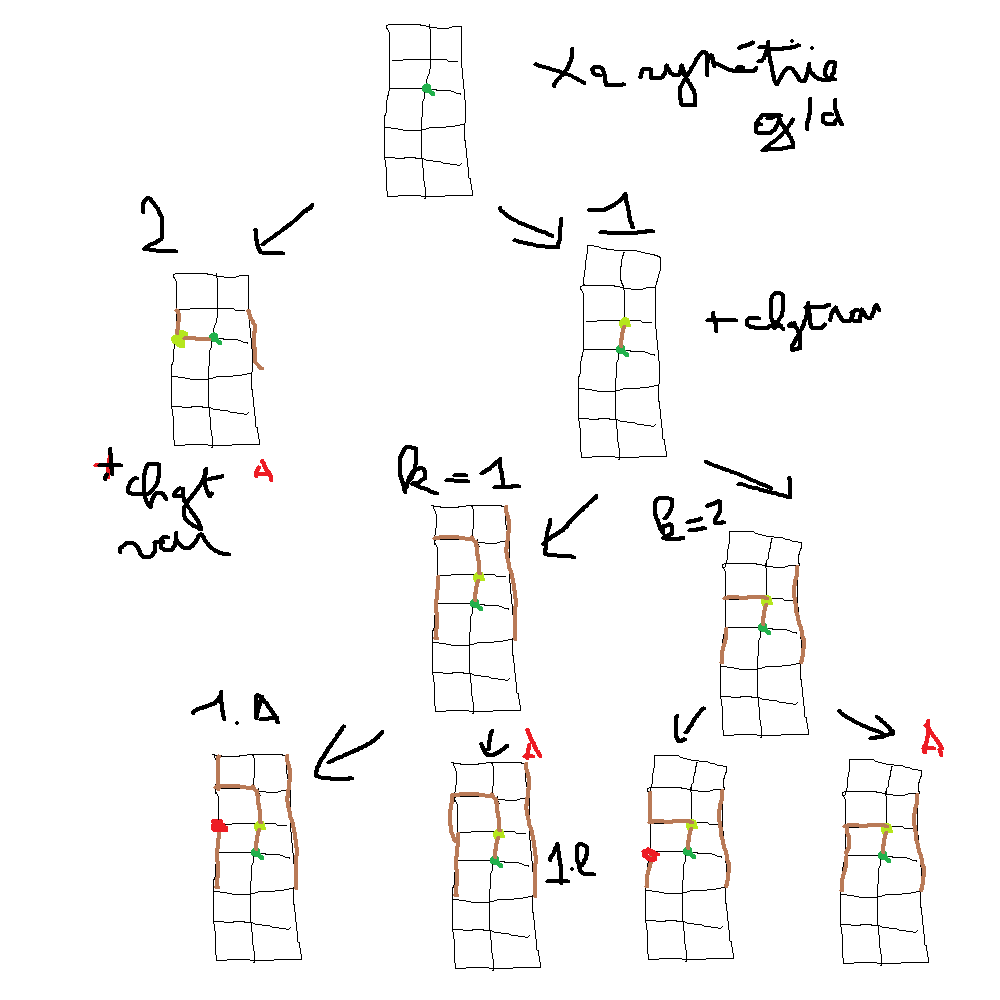
\includegraphics[angle=0, scale=0.4]{milieux_3.png}
\caption{Parcours depuis un milieu}
\label{milieux_3}
\end{figure}

En partant des dessins (cf Fig \ref{milieux_3}) qui sont même valide aux extrémités:
$$\Pm{n, h} = P_1(n, h) + P_2(n, h) $$
$$P_2(n, h) = \pb{3}{h-1} \pa{3}{n -h}$$
\begin{align}
P_1(n, h) &= P_{1a}(n, h) + P_{1l}(n, h)\\
&= \sum_{k=1}^{h-2} \pb{3}{n-h} \pb{3}{k} + \sum_{k=0}^{h-2} \pb{3}{n-h} \pa{3}{k}\\
&= \sum_{k=0}^{h-2} \pb{3}{n-h} \pb{3}{k} + \sum_{k=0}^{h-2} \pb{3}{n-h} \pa{3}{k} \quad \text{car } \pb{3}{0} = 0\\
&=  \pb{3}{n-h} \sum_{k=0}^{h-2} \pb{3}{k} \pa{3}{k}\\
\end{align}
$$\Pm{n, h} =\pb{3}{h-1} \pa{3}{n -h} + \pb{3}{n-h} \sum_{k=0}^{h-2} \pb{3}{k} \pa{3}{k}  \cqfd$$

\subsubsection{Compatibilité avec \trajet{n}{3}{1}{2}{\lambda}{\lambda} (cf  \ref{milieux_extremes})}
\begin{align}
\Pm{n, 1} &= \pb{3}{0} \pa{3}{n -1} + \pb{3}{n-h} \sum_{k=0}^{-1} \pb{3}{k} \pa{3}{k}\\
&= 0 \times 1 + \pb{3}{n} \times 0\\
&=0
\end{align}
\begin{align}
\Pm{n, n} &= \pb{3}{n-1} \pa{3}{n -n} + \pb{3}{n-n} \sum_{k=0}^{h-2} \pb{3}{k} \pa{3}{k}\\
&= \pb{3}{n-1} \times 1 + 0 \times \sum_{k=0}^{h-2} \pb{3}{k} \pa{3}{k}\\
&= \pb{3}{n-1}
\end{align}
Or
\begin{align}
\trajet{n}{3}{1}{2}{\lambda}{\lambda} = \trajet{n}{3}{n}{2}{\lambda}{\lambda} &= 2\left(\Pm{n, n} + \Pm{n, 1} \right) \\
&= 2  \pb{3}{n-1} \cqfd
\end{align}

\subsubsection{Optimisation: symétries et théorème parité}

\begin{itemize}
\item Si $2 \mid n$:
\begin{align}
\Pmtot{n} &= \sum_{h=1; 2 \nmid h}^{n}  \Pm{n, h} + \Pm{n, n -h + 1} +  \Pm{n, h+1} + \Pm{n, n - (h+1) + 1}\\
&= \sum_{h=1; 2 \nmid h}^{n - 1}  \Pm{n, h} + \Pm{n, n -h + 1} +  \Pm{n, h+1} + \Pm{n, n - h}\\
&= \sum_{h=1; 2 \nmid h}^{n - 1} P_1(n, h) + P_2(n, n-h+1) + P_2(n, h+1) + P_1(n, n-h) \cqfd
\end{align}

\begin{itemize}
\item Si $2 \mid h$:
$$\Pm{n, h} = P_1(n, h) + P_2(n, h) = P_2(n, h)$$
$$\Pm{n, n-h+1} = P_1(n, n-h+1) + P_2(n, n-h+1) = P_1(n, n-h+1)$$

\item Si $2 \nmid h$:
$$\Pm{n, h} = P_1(n, h) + P_2(n, h) = P_1(n, h)$$
$$\Pm{n, n-h+1} = P_1(n, n-h+1) + P_2(n, n-h+1) = P_2(n, n-h+1)$$
\end{itemize}

En utilisant la symétrie dans la longueur:
\begin{itemize}
\item Si $n \equiv 0 [4]$:
\begin{align}
\Pmtot{n} &= 2\sum_{h=1; 2 \nmid h}^{\frac{n}{2}-1}  \Pm{n, h} + \Pm{n, n -h + 1} +  \Pm{n, h+1} + \Pm{n, n - h}\\
&= 2\sum_{h=1; 2 \nmid h}^{\frac{n}{2}-1}  P_1(n, h) + P_2(n, n-h+1) + P_2(n, h+1) + P_1(n, n-h) \cqfd
\end{align}
\item Si $n \equiv 2 [4]$:
\begin{align}
\Pmtot{n} &=2\trajet{n}{3}{h}{2}{\lambda}{\lambda}\\
 &+2\sum_{h=1; 2 \mid h}^{\frac{n}{2}-2}  \Pm{n, h} + \Pm{n, n -h + 1} +  \Pm{n, h+1} + \Pm{n, n - h}\\
&=2P_1\left(n, \frac{n}{2}\right) + 2P_2\left(n, \frac{n}{2}\right)  \\
&+2\sum_{h=1; 2 \mid h}^{\frac{n}{2}-2} P_1(n, h) + P_2(n, n-h+1) + P_2(n, h+1) + P_1(n, n-h) \cqfd
\end{align}
\end{itemize}

\item Si $2 \nmid n$, grâce au théorème parité:
\begin{align}
\Pmtot{n} &= \sum_{h=2; 2 \mid h}^{n - 1}  \Pm{n, h} + \Pm{n, n -h + 1} +  \Pm{n, h+1} + \Pm{n, n - (h+1) + 1}\\
&= \sum_{h=2; 2 \mid h}^{n - 1}  \Pm{n, h} + \Pm{n, n -h + 1}\\
&= \sum_{h=2; 2 \mid h}^{n - 1}  P_1(n, h) + P_2(n, h) +  P_1(n, n-h+1) + P_2(n, n-h+1)
\end{align}

\begin{itemize}
\item Si $2 \mid h$:
$$\Pm{n, h} = P_1(n, h) + P_2(n, h)$$
$$\Pm{n, n-h+1} = P_1(n, n-h+1) + P_2(n, n-h+1)$$

\item Si $2 \nmid h$:
$$\Pm{n, h} = P_1(n, h) + P_2(n, h) = 0$$
$$\Pm{n, n-h+1} = P_1(n, n-h+1) + P_2(n, n-h+1) = 0$$
\end{itemize}

En utilisant la symétrie dans la longueur:
\begin{itemize}
\item Si $n \equiv 1 [4]$:
\begin{align}
\Pmtot{n} &= 2\sum_{h=2; 2 \mid h}^{\frac{n-1}{2}} \Pm{n, h} + \Pm{n, n-h+1}\\
&= 2\sum_{h=2; 2 \mid h}^{\frac{n-1}{2}} P_1(n, h) + P_2(n, h) +  P_1(n, n-h+1) + P_2(n, n-h+1) \cqfd
\end{align}
\item Si $n \equiv 3 [4]$:
\begin{align}
\Pmtot{n} 
&= 2\Pm{n, \frac{n+1}{2}} \\
&+ 2 \sum_{h=2; 2 \mid h}^{\frac{n-1}{2}} \Pm{n, h} + \Pm{n, n-h+1}\\
&= 2P_1\left(n, \frac{n+1}{2} \right) +  2P_2\left(n, \frac{n+1}{2} \right)\\
&+ 2 \sum_{h=2; 2 \mid h}^{\frac{n-1}{2}} P_1(n, h) + P_2(n, h) +  P_1(n, n-h+1) + P_2(n, n-h+1) \cqfd
\end{align}
\end{itemize}
\end{itemize}


\section{Trajets depuis les côtés: \trajet{n}{3}{\lambda}{1}{\lambda}{\lambda}}
\subsubsection{Introduction}
$$\Pctot{n} = \trajet{n}{3}{\lambda}{1}{\lambda}{\lambda} = \trajet{n}{3}{\lambda}{3}{\lambda}{\lambda}$$
$$\Pc{n, h} + \Pc{n, n-h+1} = \trajet{n}{3}{h}{1}{\lambda}{\lambda}$$

\subsubsection{Traduction en formules}
\begin{figure}[h]
\centering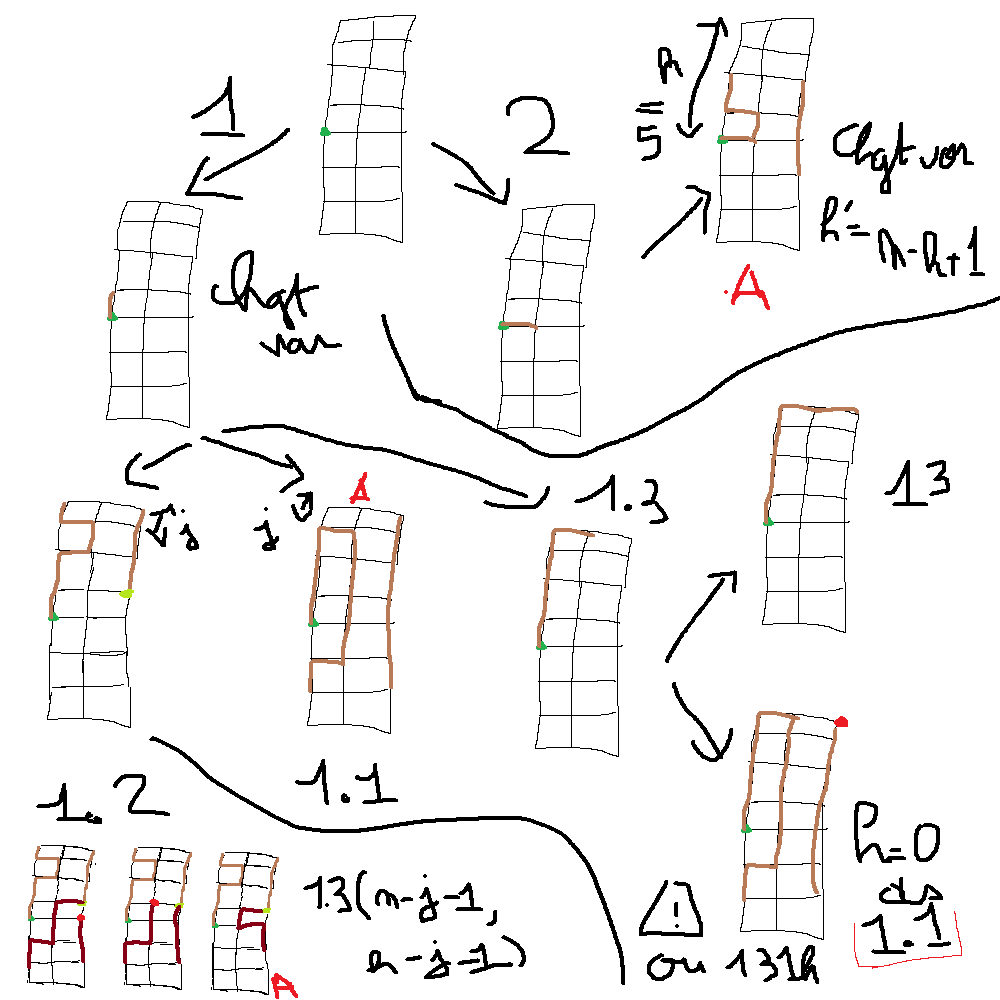
\includegraphics[angle=0, scale=0.4]{roadmap_cote.png}
\caption{Parcours depuis un côté}
\label{parcour_cote}
\end{figure}
En partant des dessins qui sont même valides aux extrémités:
$$\Pctot{n} = 2 \pa{n}{3} + \sum_{h=2}^{n-1} \Pc{n, h} + \Pc{n, n-h+1}$$
$$\Pc{n, h} = P_1(n, h) + P_2(n, h) $$

$$P_{2}(n, h) = \pb{3}{h-2} \pa{3}{n-h}$$

$$P_1(n, h) = P_{1.1}(n, h) +  P_{1.2}(n, h) + P_{1.3}(n, h)$$
$$P_{1.1} (n, h)= \sum_{k=0}^{h-2} \pb{3}{n - h - 1} \pa{3}{k} =  \pb{3}{n - h - 1} \sum_{k=0}^{h-2}\pa{3}{k}$$
$$P_{1.2}(n, h) = \sum_{k=1}^{h-3}  \pb{3}{k} P_{1.3} (n - k - 1, h- k -1)$$

\begin{figure}[h]
\centering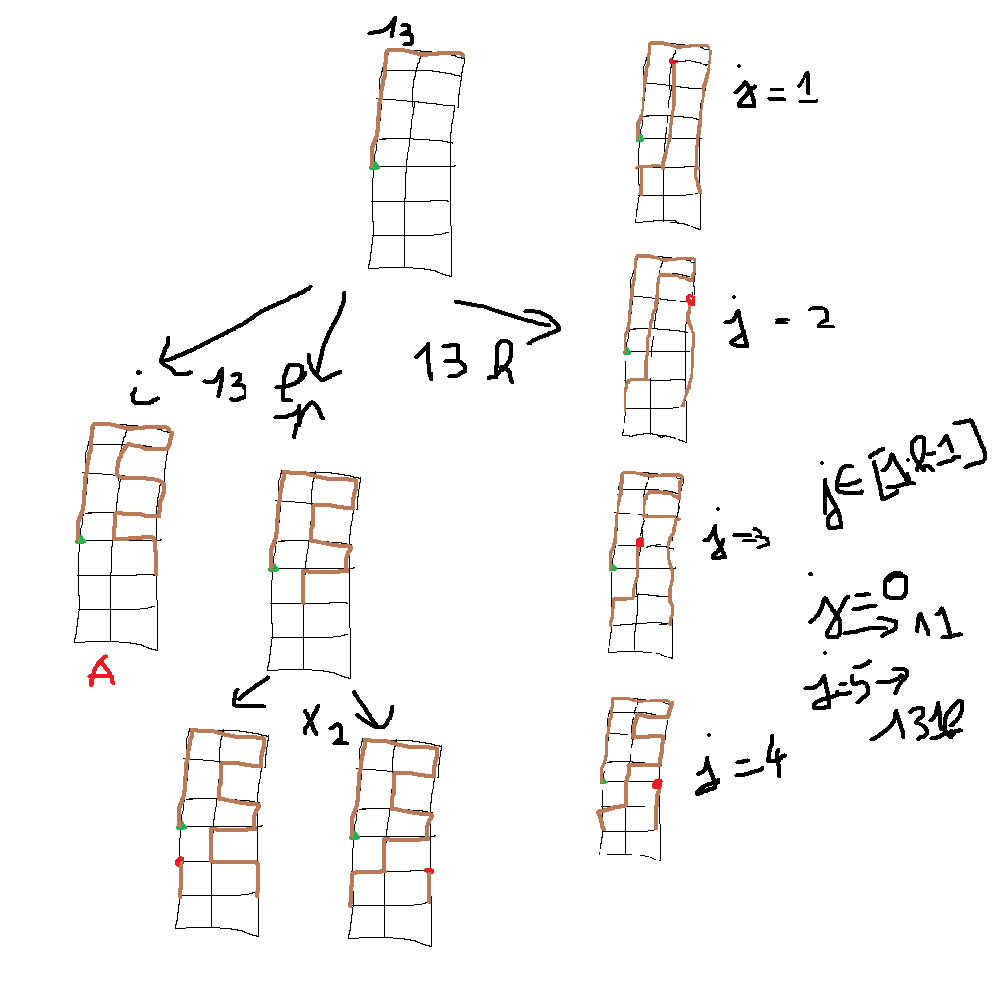
\includegraphics[angle=0, scale=0.4]{131.png}
\caption{Parcours 1.3.1}
\label{pc131}
\end{figure}

\begin{align}
P_{1.3}(n, h) &= P_{1.3.l}(n, h) + P_{1.3.h}(n, h)\\
&= P_{1.3.l}(n, h) + \sum_{k=1}^{h-1} \pb{3}{n-h-1}\\
&= P_{1.3.l}(n, h) + \sum_{k=1}^{h-1} \pb{3}{n-h-1}\\
&= P_{1.3.l}(n, h) + (h-1) \pb{3}{n-h-1}\\
\end{align}

\[
P_{1.3.l}
\left|
  \begin{array}{rcl}
    \text{Si } 2\mid h; & \quad P_{1.3.l}(n, h) =& 2 \pb{3}{n-h-1}\\
    \text{Si } 2\nmid h; & \quad P_{1.3.l}(n, h) =& \pa{3}{n-h}
  \end{array}
\right.
\]

\subsubsection{Optimisation}
\begin{itemize}

\item Si $2 \mid n$:
\begin{itemize}
\item Si $2 \mid h$:
$$P_{1.3}(n, h) =  2\pb{3}{n-h-1} + (h-1) \pb{3}{n-h-1} = (h+1) \pb{3}{n-h-1}$$

\item Si $2 \nmid h$:
$$P_{1.3}(n, h) =  \pa{3}{n-h}$$
\end{itemize}

\item Si $2 \nmid n$:
\begin{itemize}
\item Si $2 \mid h$:
$$P_{1.3}(n, h) = 0$$

\item Si $2 \nmid h$:
$$P_{1.3}(n, h) = \pa{3}{n-h} + (h-1) \pb{3}{n-h-1}$$

\end{itemize}
\end{itemize}

\newpage

\chapter[Algorithme en Python]{Algorithme en \pythonlogo}

\begin{figure}[h]%[]
\begin{lstlisting}[frame=single]
import numpy as np
from numba import jit


@jit(nopython=True)
def count_in_matrice(matrice, x, y, n):
    if not n:
        return 1
    else:
        result = 0
        for dx, dy in (1, 0), (-1, 0), (0, 1), (0, -1):
            if matrice.shape[0] > x + dx >= 0 and matrice.shape[1] > y + dy >= 0 and (not matrice[x + dx][y + dy]):
                # print(x + dx, y + dy)
                matrice[x + dx][y + dy] = True
                result += count_in_matrice(matrice, x + dx, y + dy, n - 1)
                matrice[x + dx][y + dy] = False
        return result


def walkeur(matrice, x, y):
    matrice[x][y] = True
    r = count_in_matrice(matrice, x, y, matrice.shape[0] * matrice.shape[1] - 1)
    matrice[x][y] = False
    return r
\end{lstlisting}
\caption[Algorithme de dénombrement des parcours depuis un point en Python]{Algorithme de dénombrement des parcours depuis un point en \pythonlogo}
\label{algorithme_serpent}
\end{figure}

\begin{figure}[h]%[]
\begin{lstlisting}[frame=single]
def count_path(Lx, ly):
    """Fait tt les points de depart possibles"""
    nodes = refeur(Lx, ly)
    total = 0
    if Lx % 2:  # impair
        if ly % 2:  # impair
            for x in range(0, Lx // 2):  # angle * 4
                for y in range(0, ly // 2):
                    if not (x + y) % 2:  # th parite
                        total += 4 * walkeur(coord_value(x, y, ly), Lx, ly, nodes)
            for y in range(0, ly // 2):  # reste en x
                if not (Lx // 2 + y) % 2:
                    total += 2 * walkeur(coord_value(Lx // 2, y, ly), Lx, ly, nodes)
            for x in range(0, Lx // 2):  # reste en y
                if not (ly // 2 + x) % 2:
                    total += 2 * walkeur(coord_value(x, ly // 2, ly), Lx, ly, nodes)
            if not (Lx // 2 + ly // 2) % 2:  # milieu
                total += walkeur(coord_value(Lx // 2, ly // 2, ly), Lx, ly, nodes)
        
        else:  # ly pair
            for x in range(0, Lx // 2):  # angle * 4
                for y in range(0, ly // 2):
                    total += 4 * walkeur(coord_value(x, y, ly), Lx, ly, nodes)
            for y in range(0, ly // 2):  # reste en x
                total += 2 * walkeur(coord_value(Lx // 2, y, ly), Lx, ly, nodes)
            
    else:  # Lx pair
        if ly % 2:  # impair
            for x in range(0, Lx // 2):  # angle * 4
                for y in range(0, ly // 2):
                    total += 4 * walkeur(coord_value(x, y, ly), Lx, ly, nodes)
            for x in range(0, Lx // 2):  # reste en y
                total += 2 * walkeur(coord_value(x, ly // 2, ly), Lx, ly, nodes)
            
        else:
            for x in range(0, Lx // 2):  # angle * 4
                for y in range(0, ly // 2):
                    total += 4 * walkeur(coord_value(x, y, ly), Lx, ly, nodes)
    return total

\end{lstlisting}
\caption[Algorithme de dénombrement des parcours pour un graphe en Python]{Algorithme de dénombrement des parcours pour un graphe en \pythonlogo}
\end{figure}

\begin{figure}[h]
\centering
\begin{tabular}{|c|r|c|}
\hline c & Nb parcours & Temps (s) \\
\hline 1 & 1 & 2,980E-05 \\
\hline 2 & 8 & 3,10E-05 \\
\hline 3 & 40 & 4,68E-05 \\
\hline 4 & 552 & 0,448 \\
\hline 5 & 8 648 & 0,0109 \\
\hline 6 & 458 696 & 3.656\\
\hline 7 & 27 070 560 & 1808.915 \\
\hline 8 & 6 046 626 568 & ? \\
\hline 9 &  1 490  832 682 992 & ? \\
\hline 10 & 1 460 089 659 025 264 & ? \\
\hline 11 & 1  573 342 970 540 617 696 & ? \\
\hline 12 & 6 905  329 711 608 694 708 440 & ? \\
\hline 13 & 33 304 011 435 341 069 362 631 160 & ? \\
\hline 14 & 663 618 176 813 467 308 855 850 585 056 & ? \\
\hline 15 & 14 527 222 735 920 532  980 525 200 234 503 048 & ? \\
\hline 16 & 1 325 269 434 769 959 586 477 628 202 755 977 573 768 & ? \\
\hline 17 & 132 857 989 478 318 939 938 880 239 159 473 615 225 331 080 & ? \\
\hline
\end{tabular}
\caption[Nombre de parcours]{Résultats de l'algorithme et de l'OEIS}
\label{tableau_resultats_serpent}
\end{figure}

% \listtheoremname[ignoreall,show={theorem,defn}]
\listoffigures
\setcounter{tocdepth}{5}
\tableofcontents
%\listtheorems[ignoreall,show={theorem,defn}]
\end{document}